\normaltrue
\correctionfalse

%\UPSTIidClasse{11} % 11 sup, 12 spé
%\newcommand{\UPSTIidClasse}{12}

\exer{Mouvement T -- $\star$ \label{DYN:05:B2:13:01:02}}
\setcounter{question}{0}\marginnote{\xpComp{DYN}{05}}%\UPSTIcompetence{B2-13}
\index{Compétence B2-13}\index{Compétence DYN-05}
\index{Mécanisme à 1 translation}
\ifcorrection
\else
\marginnote{\textbf{Pas de corrigé pour cet exercice.}}
\fi

\ifprof
\else
Soit le mécanisme suivant. On note $\vect{AB}=\lambda(t)\vect{i_0}$.
\begin{marginfigure}
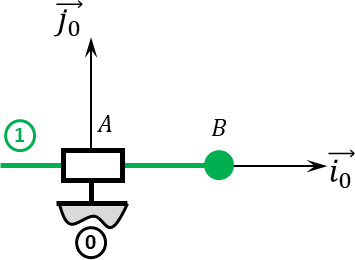
\includegraphics[width=.6\linewidth]{01_T_01}
\end{marginfigure}
\fi

\question{Donner le torseur cinématique $\torseurcin{V}{1}{0}$ au point $B$.}
\ifprof
\else
\fi

\question{Déterminer $\vectg{B}{1}{0}$.}
\ifprof
\else
\fi


\ifprof
\else

\marginnote{Corrigé voir \ref{DYN:05:B2:13:01:02}.}

\fi


